% Title: gl2ps_renderer figure
% Creator: GL2PS 1.4.2, (C) 1999-2020 C. Geuzaine
% For: Octave
% CreationDate: Tue Sep 28 14:08:51 2021
\setlength{\unitlength}{1pt}
\begin{picture}(0,0)
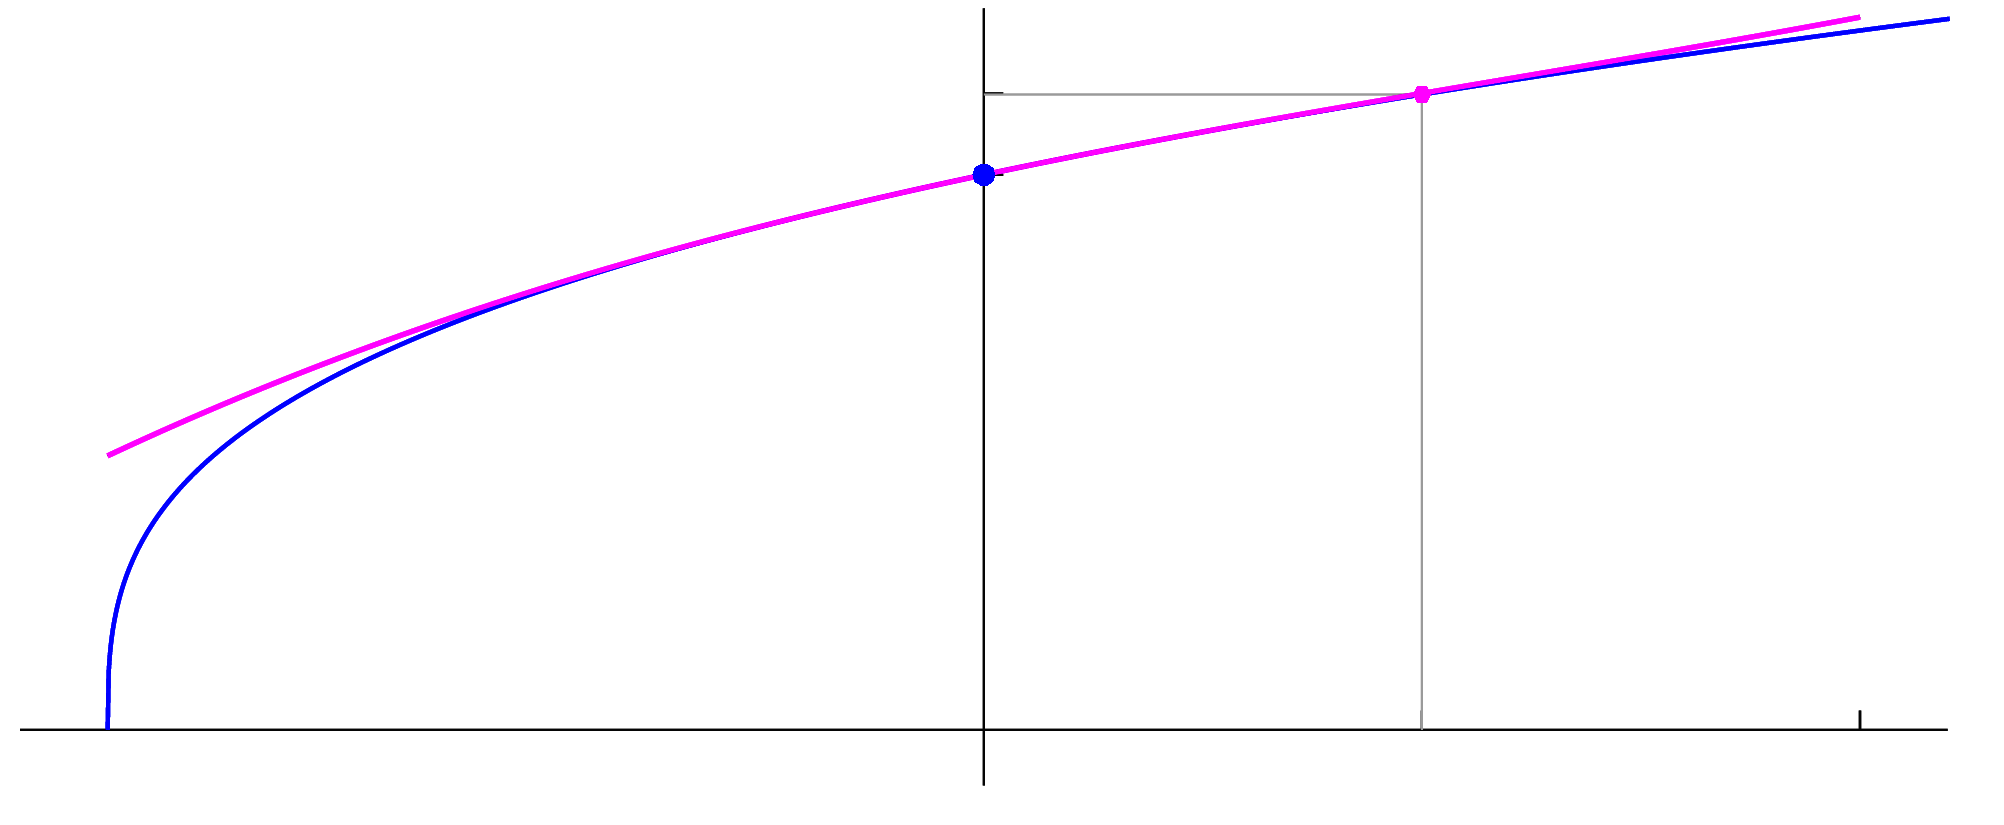
\includegraphics[width=17cm,height=7cm]{fig_taylor_sqrt3}
\end{picture}%
\begin{picture}(481,198)(0,0)
\fontsize{10}{0}\selectfont\put(25.8468,15.3382){\makebox(0,0)[t]{\textcolor[rgb]{0.15,0.15,0.15}{{-1,0}}}}
\fontsize{10}{0}\selectfont\put(341.266,15.3382){\makebox(0,0)[t]{\textcolor[rgb]{0.15,0.15,0.15}{{0,5}}}}
\fontsize{10}{0}\selectfont\put(446.405,15.3382){\makebox(0,0)[t]{\textcolor[rgb]{0.15,0.15,0.15}{{1,0}}}}
\fontsize{10}{0}\selectfont\put(231.13,156.047){\makebox(0,0)[r]{\textcolor[rgb]{0.15,0.15,0.15}{{1}}}}
\fontsize{10}{0}\selectfont\put(231.13,175.579){\makebox(0,0)[r]{\textcolor[rgb]{0.15,0.15,0.15}{{1,1466}}}}
\fontsize{10}{0}\selectfont\put(36.3608,109.417){\makebox(0,0)[l]{\textcolor[rgb]{0,0,0}{{$P_3$}}}}
\fontsize{10}{0}\selectfont\put(32.1552,49.4646){\makebox(0,0)[l]{\textcolor[rgb]{0,0,0}{{$\sqrt[3]{1+x}$}}}}
\end{picture}
